\documentclass{report}
% PACKAGES %
\usepackage[english]{} % Sets the language
\usepackage[margin=2cm]{geometry} % Sets the margin size
\usepackage{graphicx} % Enhanced package for including graphics/figures
\usepackage{float} % Allows figures and tables to be floats
\usepackage{amsmath} % Enhanced math package prepared by the American Mathematical Society
\usepackage{amssymb} % AMS symbols package
\usepackage{bm} % Allows you to use \bm{} to make any symbol bold
\usepackage{verbatim} % Allows you to include code snippets
\usepackage{setspace} % Allows you to change the spacing between lines at different points in the document
\usepackage{parskip} % Allows you alter the spacing between paragraphs
\usepackage{multicol} % Allows text division into multiple columns
\usepackage{units} % Allows fractions to be expressed diagonally instead of vertically
\usepackage{booktabs,multirow,multirow} % Gives extra table functionality
\usepackage{enumerate}
\newcommand{\tab}{\-\hspace{1.5cm}}

% Set path to figure image files
\graphicspath{ {fig/} }

\begin{document}

\begin{center}
\textbf{\large Nuclear Engineering 150 -- Discussion Section}\\ 
\textbf{Team Exercises \#13}
\end{center}

%%%%%%%%%%%%%%%%%%%%%%%%%%%%%%%%%% PROBLEM 1 %%%%%%%%%%%%%%%%%%%%%%%%%%%%%%%%%%
\section*{Problem 1}

A homogeneous U-235 reactor is operating at full power, 10,000 W/cm$^3$. 13\% of neutrons are absorbed in resonances, 2\% of all fission events are fast fissions, and 10\% of neutrons leak from the reactor. Assume 2.4 neutrons and 200 MeV are produced per fission, the fission cross section is 0.6 cm$^{-1}$, and the absorption cross section is 1 cm$^{-1}$.
\begin{enumerate}[a)]
\item Ignoring depletion, calculate the excess reactivity of this reactor.
\item The reactor scrams (immediately jumps to zero power). The plot below gives the negative reactivity as a function of time due to the accumulation of xenon in the reactor. Estimate at which point the reactor could no longer be returned to operation. About how long would this deadtime last?
\end{enumerate}
\begin{center}
\vspace{1cm}
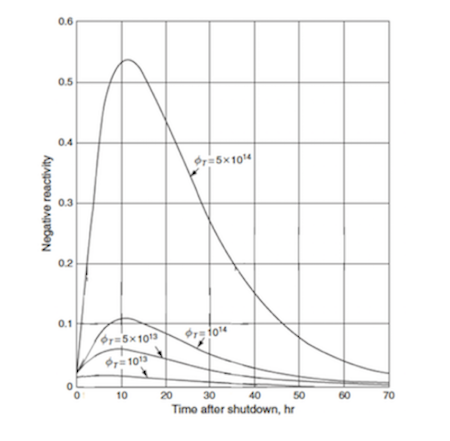
\includegraphics[width=12cm]{xenon-deadtime}
\end{center}
\vfill
$200\text{ MeV} = 3.204\times10^{-11}\text{ J}$



\newpage
%%%%%%%%%%%%%%%%%%%%%%%%%%%%%%%%%% PROBLEM 2 %%%%%%%%%%%%%%%%%%%%%%%%%%%%%%%%%%
\section*{Problem 2}

Three unknown fission products $A$, $B$ and $C$ are produced by a reactor. $B$ is stable and has a very large absorption cross section at the energies found in the reactor. The population of isotope $B$ is fed by other known fission products. Isotope $C$ decays relatively quickly into isotope $A$, which then decays again in short order. $C$ has a neglible absorption cross section, while $A$'s cross section is large. 

For each isotope, plot the behavior of the isotope's concentration after the reactor is turned on, left for a long time, then first dropped to some non-zero power, and finally shut-down.



\end{document}
